% A labeled short box with an explicit width and height (shorter than \shortanswerbox).
\newcommand{\gridbox}[3]{%
  \ifthenelse{\equal{\version}{solution}}{%
    \tikz[baseline=(x.base)]\draw (0,0) rectangle node (x) [text width=\dimexpr#1-6pt\relax, align=left] {\scriptsize #3} (#1, #2);%
  }{%
    \tikz[baseline=(x.base)]\draw (0,0) rectangle node (x) {\vphantom{Aq}} (#1, #2);%
  }}
\par\vspace{2ex}\noindent\begin{minipage}{\linewidth}
\section*{Threat Models and Foundations}

\prob{4} An AI agent that posts class announcements holds a stored Slack token. An
attacker obtains the token and posts ``The midterm is canceled'' to the course
channel. Give the threat model, one item per box: the {\bf asset} harmed (not the
token itself), the {\bf property} violated, a plausible {\bf adversary} and their
motive, and the {\bf capability} the attacker needed.

\vspace{4pt}
\begin{tabular}{@{}p{0.72in}p{2.45in}p{0.85in}p{2.45in}@{}}
Asset: & \gridbox{6cm}{1.8cm}{the channel; the instructor's voice} & Property: & \gridbox{6cm}{1.8cm}{integrity (accept authenticity)} \\[8pt]
Adversary: & \gridbox{6cm}{1.8cm}{a prankster or a student wanting a delay} & Capability: & \gridbox{6cm}{1.8cm}{the stored token: acts as the instructor, no second factor} \\
\end{tabular}
\eprob
\end{minipage}\par

\par\noindent\begin{minipage}{\linewidth}
\prob{3} Every security system has a {\em root of trust}: the point where the
chain of trust stops and you simply accept something. For each, name the key or
certificate that is accepted without being checked, and who ships it.

\vspace{4pt}
\begin{tabular}{@{}p{3.0in}p{3.5in}@{}}
A browser's TLS connection to a web site: & \gridbox{8.8cm}{1.5cm}{the root CAs shipped with the OS or browser (accept the vendor that ships the root store)} \\[10pt]
DNSSEC validation of a DNS answer: & \gridbox{8.8cm}{1.5cm}{the root zone's public key built into the resolver software} \\[10pt]
RPKI's check that an AS may announce a prefix: & \gridbox{8.8cm}{1.5cm}{the regional registries' trust-anchor keys in the validator (accept IANA/ICANN as the top of the delegation)} \\
\end{tabular}
\eprob
\end{minipage}\par

\par\noindent\begin{minipage}{\linewidth}
\prob{3} A payments startup discovers that a production API key committed to a
public GitHub repository eight months ago has been used by an outsider to issue
refunds. Among the failure modes in Anderson's ``Why Cryptosystems Fail,'' this is
primarily a failure of: (Select the best answer.)\\
\answercircle{The cryptographic algorithm protecting the key}\\
\correctanswercircle{Key management and operational procedure}\\
\answercircle{A remote software vulnerability in the API server}\\
\answercircle{A fake terminal or skimmer}\\
\answercircle{Usability of the customer-facing product}
\eprob
\end{minipage}\par

\par\noindent\begin{minipage}{\linewidth}
\prob{4} {\bf Case study.} In 2012 an anonymous researcher logged into hundreds of
thousands of home routers that still had their factory default passwords, used
them to scan the entire Internet, and published the data set (the ``Carna
botnet''). The owners were never asked. Today a graduate student proposes to use
the published data set to study how address usage has changed since 2012. Using
{\em respect for persons}, give one argument {\bf against} the original
collection; using {\em beneficence}, give one argument {\bf for} the reuse today.

\begin{tabular}{@{}p{3.15in}p{3.15in}@{}}
Against the collection (respect for persons): & For the reuse (beneficence): \\
\gridbox{7.8cm}{2.4cm}{The owners' devices were accessed and modified without informed consent: never asked, never told, no way to opt out, so they were treated as means rather than persons.} & \gridbox{7.8cm}{2.4cm}{The data already exists and cannot be un-collected; reuse adds no new risk to the owners (decade-old address-level data) and the benefit, a baseline for Internet growth, is real; risk against benefit favors reuse even though it did not favor collection.} \\
\end{tabular}
\eprob
\end{minipage}\par

\par\vspace{1.2ex}\noindent\begin{minipage}{\linewidth}
\section*{Key Management and Public Key Infrastructure}

\prob{4} Which of the following statements are true? (Select all that apply.)\\
\correctanswercircle{A browser uses asymmetric cryptography to establish a symmetric key, which then encrypts the traffic}\\
\correctanswercircle{To send Bob a message only he can read, Alice encrypts it with Bob's public key}\\
\answercircle{To sign a message so others can verify it came from her, Alice uses Bob's public key}\\
\correctanswercircle{A certificate is a signed statement binding an identity to a public key, with an issuer and validity period}\\
\answercircle{Integrity means that only authorized parties can read a message}
\eprob
\end{minipage}\par

\par\noindent\begin{minipage}{\linewidth}
\prob{4} The first time you connect to a new server with SSH, the client shows a
key fingerprint and asks whether to trust it. Explain how Mallory, on the network
path, mounts a man-in-the-middle attack on that first connection, and what a
careful user must do to defeat it.

\answerbox{1.0}{
\small The client has no prior key, so Mallory intercepts the connection, presents her own key and fingerprint, and connects onward to the real server as the client; she shares one session key with each side and reads and re-encrypts everything. Defeat: confirm the fingerprint out of band over a channel Mallory does not control (the admin's web page, a phone call, a key published in advance); afterwards known-hosts pins the key.
}
\eprob
\end{minipage}\par

\par\noindent\begin{minipage}{\linewidth}
\prob{4} In Assignment 1 you captured your own HTTPS traffic with Wireshark and
served your site with a self-signed certificate.

\begin{tabular}{@{}p{3.15in}p{3.15in}@{}}
\small (a) Even though the payload was encrypted, name {\bf two} things an on-path eavesdropper could still learn from an HTTPS connection like the one you captured. & \small (b) The browser warned about your self-signed certificate until you took one step. What was it, and what could someone who performed that same step on your laptop without your knowledge then do to your {\em other} HTTPS traffic? \\
\gridbox{7.8cm}{2.4cm}{Visible: SNI in the ClientHello; the server's and client's IP addresses; sizes and timing of records; the preceding DNS query. Any two.} & \gridbox{7.8cm}{2.4cm}{Add the certificate to the machine's (or browser's) trust store, making it a root of trust. Anyone who can install a root on your machine can mint a certificate for any site and sit on the path as a man in the middle with no browser warning.} \\
\end{tabular}
\eprob
\end{minipage}\par

\par\noindent\begin{minipage}{\linewidth}
\prob{3} Alice posts her public key in the course Slack channel so people can
send her encrypted mail. This solves the key-distribution problem for anyone who
wants to write to her. \yesnono\ Explain why or why not.

\answerbox{1.0}{
\small No. Anyone who can post as Alice, alter the message, or sit between the reader and the channel can substitute their own key, and the reader cannot tell. Distribution needs a trusted binding of identity to key (a certificate from a party already trusted, a fingerprint confirmed out of band, a pinned key), not just a place to post it. Partial credit for Yes: posting a public key does remove the $n^2$ shared-key part of the problem (one key pair each instead of a shared key per pair); what it does not solve is binding the key to Alice.
}
\eprob
\end{minipage}\par

\par\vspace{1.2ex}\noindent\begin{minipage}{\linewidth}
\section*{Authentication and Access Control}

\prob{4} A desktop AI assistant asks to read the files in your Dropbox. The diagram
shows the OAuth flow between four parties, A through D. OAuth names four roles:
{\bf resource owner}, {\bf client}, {\bf authorization server}, and {\bf resource
server}. Write the letter of the party that plays each role.\par\noindent\begin{minipage}[t]{0.40\linewidth}
\vspace{0pt}
\begin{tabular}{@{}p{1.45in}p{0.8in}@{}}
Resource owner: & \gridbox{1.4cm}{0.9cm}{A} \\[2pt]
Client: & \gridbox{1.4cm}{0.9cm}{B} \\[2pt]
Authorization server: & \gridbox{1.4cm}{0.9cm}{C} \\[2pt]
Resource server: & \gridbox{1.4cm}{0.9cm}{D} \\
\end{tabular}
\end{minipage}\hfill
\begin{minipage}[t]{0.57\linewidth}
\vspace{0pt}
\ifthenelse{\equal{\version}{solution}}{%
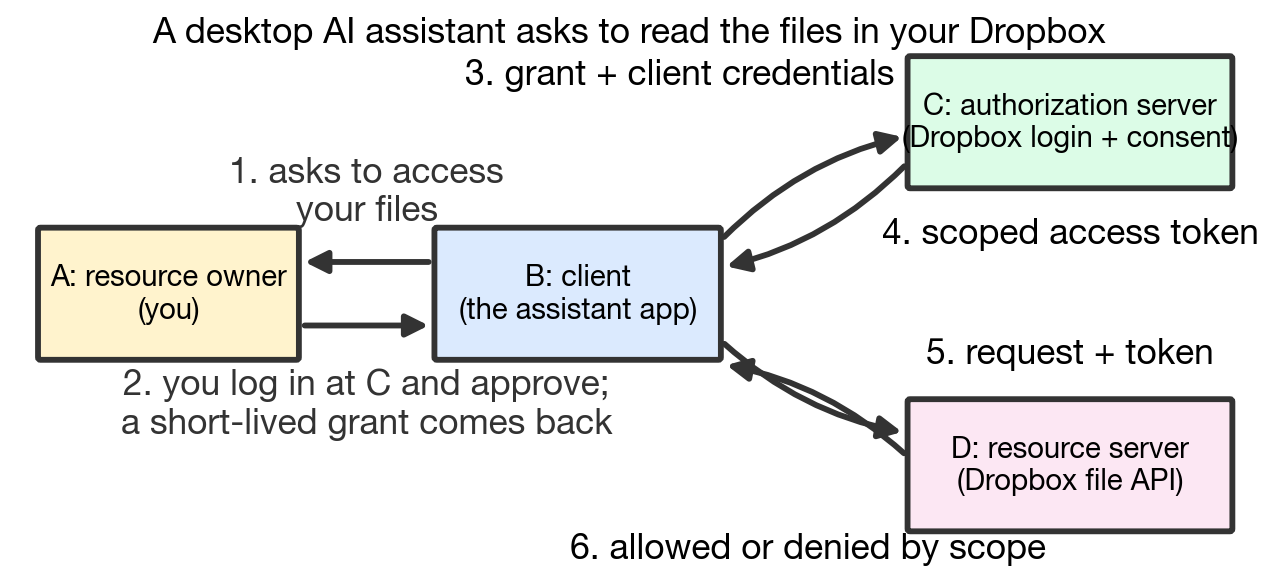
\includegraphics[width=\linewidth]{oauth-roles-solution.png}%
}{%
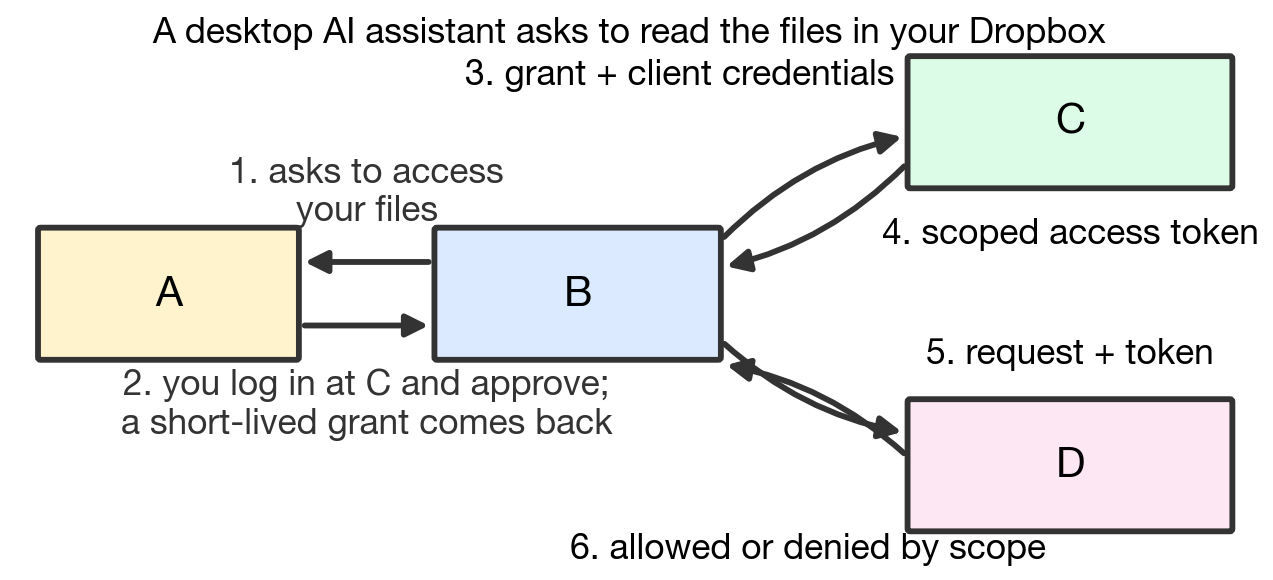
\includegraphics[width=\linewidth]{oauth-roles.png}%
}
\end{minipage}
\eprob
\end{minipage}\par

\par\noindent\begin{minipage}{\linewidth}
\prob{3} The agent that posts the class agenda presents a token to Slack, which
checks the token and then lets it post in one channel but not delete messages.
Which statements use the right term? (Select all that apply.)\\
\correctanswercircle{Presenting the token and having Slack verify it is {\em authentication}}\\
\answercircle{Presenting the token is {\em authorization}; checking it is {\em identification}}\\
\correctanswercircle{Allowing posting but not deletion is {\em authorization}, enforced by access control}\\
\answercircle{Allowing posting but not deletion is {\em authentication}}\\
\correctanswercircle{Recording that the agent posted at 3:05 pm is {\em logging}, which supports accountability}
\ifthenelse{\equal{\version}{solution}}{\par\small\textbf{Grading note:} the first option is ambiguous (the token is an authorization credential, so checking it can be read as authorization; read with commas, it is authentication). It is credited whether marked or blank.}{}
\eprob
\end{minipage}\par

\par\noindent\begin{minipage}{\linewidth}
\prob{3} A budgeting app offers to track your spending if you give it your username
and password for your bank's web site.

\noindent (a) Explain why this violates least privilege.\par
\answerbox{0.9}{
\small With your password the app can do anything you can (read every account, move money, change settings) and looks like you in every log; it cannot be limited, audited, or revoked short of a password change. Least privilege: grant only what the task needs.
}

\noindent (b) Describe the narrow OAuth scope the bank should grant instead, as {\bf who} (subject) may do {\bf what} (verb) to {\bf which data} (object).\par
\begin{tabular}{@{}p{0.6in}p{1.6in}p{0.5in}p{1.0in}p{0.6in}p{1.9in}@{}}
Subject: & \gridbox{4cm}{0.9cm}{the budgeting app (accept ``the app acting for the user'')} & Verb: & \gridbox{2.4cm}{0.9cm}{read (only); accept ``track'' or ``view''} & Object: & \gridbox{4.6cm}{0.9cm}{transactions and balances on the accounts the user selects} \\
\end{tabular}
\eprob
\end{minipage}\par

\par\vspace{1.2ex}\noindent\begin{minipage}{\linewidth}
\section*{Denial of Service}

\prob{4} To stop a denial-of-service attack coming from one region, campus IT
installs a firewall at the edge of the network that inspects every incoming
connection and drops the attack traffic. Deploying the firewall has introduced a
{\bf new} denial-of-service vulnerability. \yesnoyes\ Explain why or why not.

\answerbox{1.0}{
\small Yes. The firewall has finite memory and CPU, and every packet, including all the attack traffic, must now pass through it and be inspected. Enough traffic exhausts its state table or CPU, and when it fails nobody gets through, so the appliance added to stop the attack is the new, easier target. Any device placed in front of a service becomes the next finite resource to exhaust.
}
\eprob
\end{minipage}\par

\par\noindent\begin{minipage}{\linewidth}
\prob{4} A new chat service allocates a 64\,KB message buffer for every connection
request the moment it arrives, before the client has sent anything else. Describe
one way an attacker exploits this, and redesign the protocol in the spirit of SYN
cookies so that the attack no longer works. A sentence or two of design is enough; no
cryptographic detail is needed.

\answerbox{1.1}{
\small Exploit: flood the server with connection requests from spoofed or throwaway sources and never follow up; each costs the attacker one small packet and the server 64 KB, so memory runs out first. Redesign: do no work on the first packet; reply with a small cookie derived from the client's address and a secret, and allocate the buffer only when the client returns it, proving it is real and reachable. The client spends effort before the server does.
}
\eprob
\end{minipage}\par

\par\vspace{1.2ex}\noindent\begin{minipage}{\linewidth}
\section*{Routing Security}

\prob{2} YouTube announces its addresses as a /22. Pakistan Telecom, intending to
block YouTube inside Pakistan, announces two /24s covering the same space, and the
announcement leaks to the whole Internet. Why did the world's YouTube traffic go
to Pakistan? (Select the best answer.)\\
\answercircle{Pakistan Telecom's AS path was shorter}\\
\correctanswercircle{Routers prefer the more specific (longer) prefix, so the /24s won over the /22}\\
\answercircle{YouTube's RPKI certificate had expired}\\
\answercircle{Pakistan Telecom signed its announcement with BGPsec}
\eprob
\end{minipage}\par

\par\noindent\begin{minipage}{\linewidth}
\prob{3} Name {\bf two} different things an attacker can do with someone else's
addresses or traffic once a hijacked announcement is believed.

\answerbox{0.9}{
\small Eavesdrop on the traffic; black-hole it (denial of service, as Pakistan did); forward it to the real destination as a man in the middle (needs a path to the destination); or use hijacked, unused space as a disposable source for spam, then withdraw the route to defeat address-based block lists. Any two.
}
\eprob
\end{minipage}\par

\par\noindent\begin{minipage}{\linewidth}
\prob{4} In BGPsec, each AS signs an attestation covering the AS path so far
{\bf and the AS it is sending the announcement to}. AS 160 originates a prefix and announces it to AS 174, which announces it to
AS 15169. Suppose each AS signed the path so far but {\bf not} the AS it was sending
the announcement to. What could a dishonest AS 15169 announce to its own neighbors
that would still pass validation, and why does 160's signature naming 174 prevent it?

\answerbox{1.2}{
\small Signing only one's own hop lets AS 15169 drop 174 from the announcement it received and re-announce 160 then 15169 with the origin's genuine signature intact: a shorter path with a correct origin, so origin validation passes. With the next hop signed, 160's attestation says ``to 174''; a path omitting 174 would need 160 to have signed ``to 15169'', which it never did and 15169 cannot forge.
}
\eprob
\end{minipage}\par

\par\vspace{1.2ex}\noindent\begin{minipage}{\linewidth}
\section*{Web Security}

\prob{3} A page is loaded from \texttt{https://www.cs.uchicago.edu/courses}. Which of
the following share its {\bf origin} under the same-origin policy? (Select all that
apply.)\\
\correctanswercircle{\texttt{https://www.cs.uchicago.edu/people}}\\
\answercircle{\texttt{http://www.cs.uchicago.edu/courses}}\\
\answercircle{\texttt{https://cs.uchicago.edu/courses}}\\
\correctanswercircle{\texttt{https://www.cs.uchicago.edu/courses?term=autumn}}\\
\correctanswercircle{A script the page loads from \texttt{https://cdn.example.com/jquery.js} runs in the page's origin}
\eprob
\end{minipage}\par

\par\noindent\begin{minipage}{\linewidth}
\prob{3} A web application runs the pseudocode\\
\texttt{run\_shell("ls " + request.parameter("dir"))}\\
when a user requests a directory listing. What class of vulnerability is this, and what would an attacker
put in the \texttt{dir} parameter to make the server run a command of the attacker's
choosing? (An English description of the value is fine.)

\answerbox{1.15}{
\small Shell (command) injection: request data is pasted into a command and the shell cannot tell data from code. A dir value such as ``; <command>'' (any separator such as a semicolon or a pipe, followed by the attacker's command: a reverse shell, reading a password file, deleting files) runs ls and then that command with the web application's permissions. Fix: never build commands from strings; allow-list the value or pass it as an argument, not through a shell.
}
\eprob
\end{minipage}\par

\par\noindent\begin{minipage}{\linewidth}
\prob{3} A discussion forum displays each comment exactly as the author typed it,
and a user posts a comment containing a \texttt{<script>} tag. Is this
\answercircle{reflected} or \correctanswercircle{stored} cross-site scripting? Why
does the same-origin policy not protect the forum's other users?

\answerbox{1.15}{
\small Stored. The same-origin policy does not help because the forum itself delivers the script, so it runs in the forum's origin with full access to its DOM, cookies, and storage; the policy separates origins, but the attacker's code is inside the trusted one.
}
\eprob
\end{minipage}\par

\par\noindent\begin{minipage}{\linewidth}
\prob{3} You are logged in to your bank in one tab and visit a page showing a
picture of a muffin in another.

\noindent (a) What kind of attack can the muffin page mount against your bank account,
and why does it work?\par
\answerbox{1.05}{
\small Cross-site request forgery: the muffin page embeds a hidden image or request whose URL is a bank action, and the browser attaches your bank session cookie because it sends a domain's cookies with every request to that domain, whatever page caused it.
}

\noindent (b) Name one defense that stops it: \gridbox{10.5cm}{1.1cm}{a per-session token in the bank's own forms (unreadable to the muffin page under the same-origin policy), or SameSite cookies, now the default, which are withheld on cross-site subresource requests and POSTs}
\eprob
\end{minipage}\par

\par\vspace{1.2ex}\noindent\begin{minipage}{\linewidth}
\section*{Web Privacy}

\prob{3} \texttt{nytimes.com} and \texttt{walmart.com} both embed a script from
\texttt{tracker.example}. Explain how \texttt{tracker.example} learns that the same
person visited both sites.

\answerbox{1.2}{
\small On the first visit the script sets a tracker.example cookie holding an identifier. On every later page embedding the script, the browser (1) sends that cookie back automatically, because a domain's cookies go with every request to that domain whatever page caused it, and (2) sends a Referer header naming the page. The tracker sees the same identifier arrive from nytimes.com and then walmart.com. Accept any two of: fetching embedded third-party resources automatically, sending the tracker's cookie with every request to its domain, sending Referer (or the script reporting the page URL).
}
\eprob
\end{minipage}\par

\par\noindent\begin{minipage}{\linewidth}
\prob{3} You are not signed in to any account, you have deleted all your cookies,
and you use a private-browsing window. A tracking script embedded on the sites
you visit can still recognize that your visits come from the same browser.
\yesnoyes\ Explain why or why not.

\answerbox{1.0}{
\small Yes. The script can fingerprint the browser with no stored state: user-agent, fonts, plugins, screen size, time zone, canvas rendering combine into a value that is unique or nearly so (one in hundreds of thousands in the class demo). It is recomputed on every visit, so deleting cookies and staying signed out does not reset it; the tracker can even re-create the cookie.
}
\eprob
\end{minipage}\par

\par\vspace{1.2ex}\noindent\begin{minipage}{\linewidth}
\section*{DNS Security and Privacy}

\prob{3} Which of the following statements are true? (Select all that apply.)\\
\answercircle{DNSSEC provides confidentiality: an eavesdropper cannot see which names you look up}\\
\correctanswercircle{Encryption provides confidentiality; signatures provide integrity}\\
\answercircle{A browser cannot resolve names itself; every lookup must go through the operating system's stub resolver}\\
\correctanswercircle{With Oblivious DNS, no single server sees both your address and your query}\\
\correctanswercircle{DNS-over-HTTPS moves trust from your network operator to the resolver provider rather than eliminating it}
\eprob
\end{minipage}\par

\par\noindent\begin{minipage}{\linewidth}
\prob{3}\par\noindent\begin{minipage}[t]{0.36\linewidth}
\vspace{0pt}
The diagram shows a lookup of \texttt{www.foo.com} with nothing cached.
\begin{enumerate}[leftmargin=*,itemsep=0pt,topsep=2pt]
\item[(a)] In each dashed box, label message 3, 5, 7, or 8 with {\bf R} if it is a referral to another server or {\bf A} if it is an answer carrying the record.
\item[(b)] Draw a box around the link (both directions) that DNS-over-HTTPS encrypts.
\end{enumerate}
\end{minipage}\hfill
\begin{minipage}[t]{0.62\linewidth}
\vspace{0pt}
\ifthenelse{\equal{\version}{solution}}{%
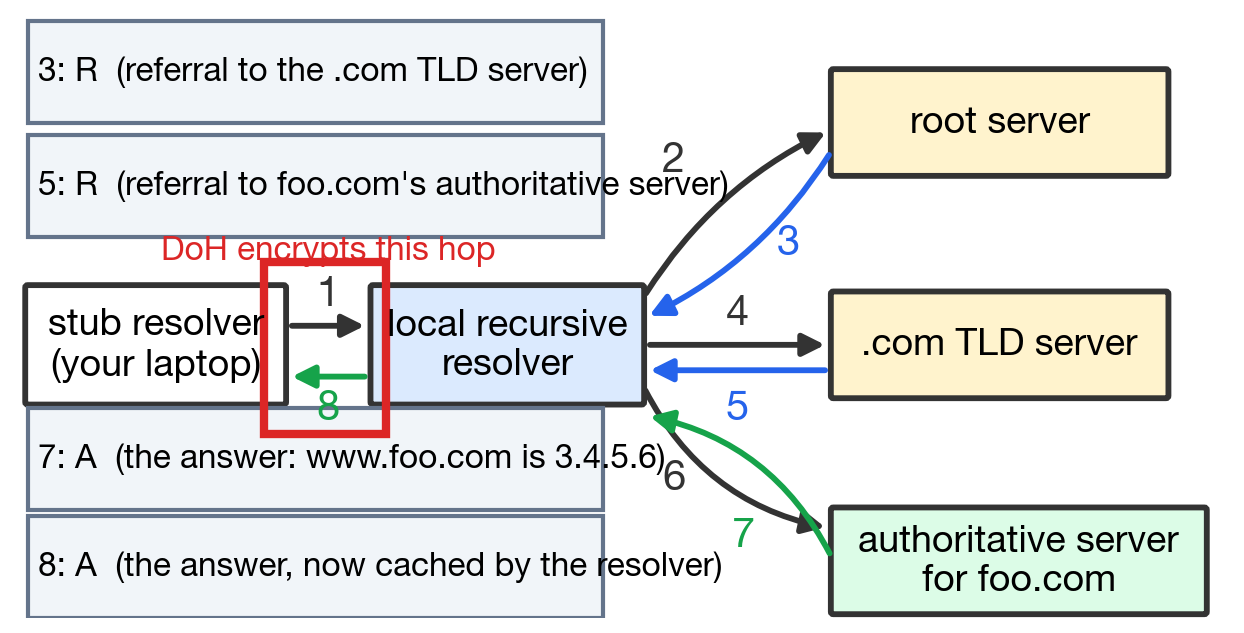
\includegraphics[width=0.8\linewidth]{dns-lookup-solution.png}%
}{%
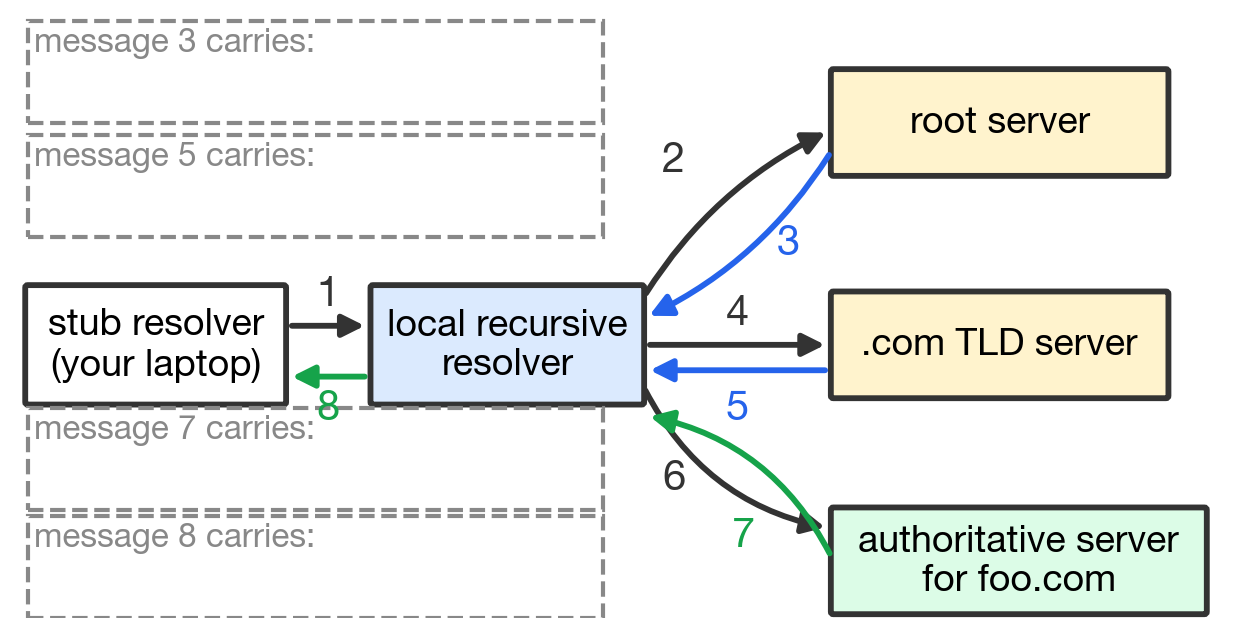
\includegraphics[width=0.8\linewidth]{dns-lookup.png}%
}
\end{minipage}
\eprob
\end{minipage}\par

\par\noindent\begin{minipage}{\linewidth}
\prob{3}\par\noindent\begin{minipage}[t]{0.46\linewidth}
\vspace{0pt}
The resolver's cache entry for \texttt{google.com} has expired; it re-queries the
authoritative server with transaction ID \texttt{0x3a7f}, which the {\bf off-path}
attacker cannot see. In the dashed box, write what the attacker sends (its content,
and how many); below, explain in one sentence why it works.\\[0.5ex]
\answerbox{1.4}{
\small Forged answers (google.com = 6.6.6.6) with every 16-bit ID, all 65,536 (accept ``every possible ID''), spoofed from the authoritative server's address. The ID is the resolver's check, and the attacker can enumerate every ID without seeing the query; one that matches and beats the real reply is cached. Credit answers that add source spoofing or the race.
}
\end{minipage}\hfill
\begin{minipage}[t]{0.52\linewidth}
\vspace{0pt}
\ifthenelse{\equal{\version}{solution}}{%
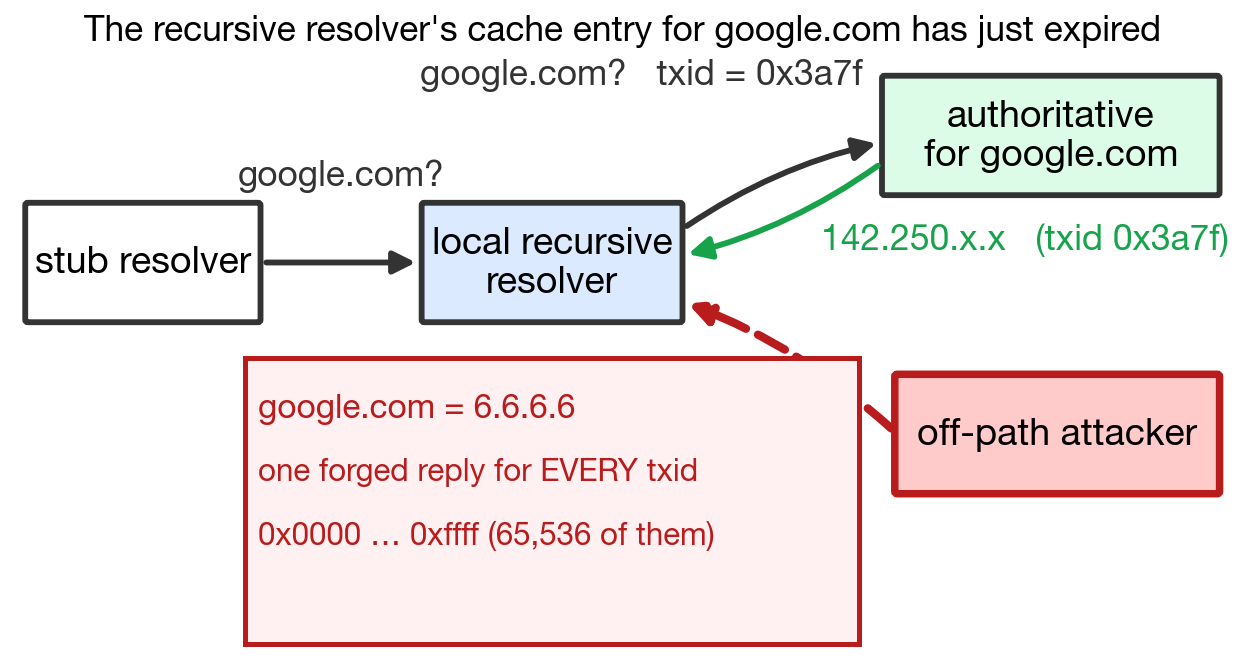
\includegraphics[width=\linewidth]{kaminsky-solution.png}%
}{%
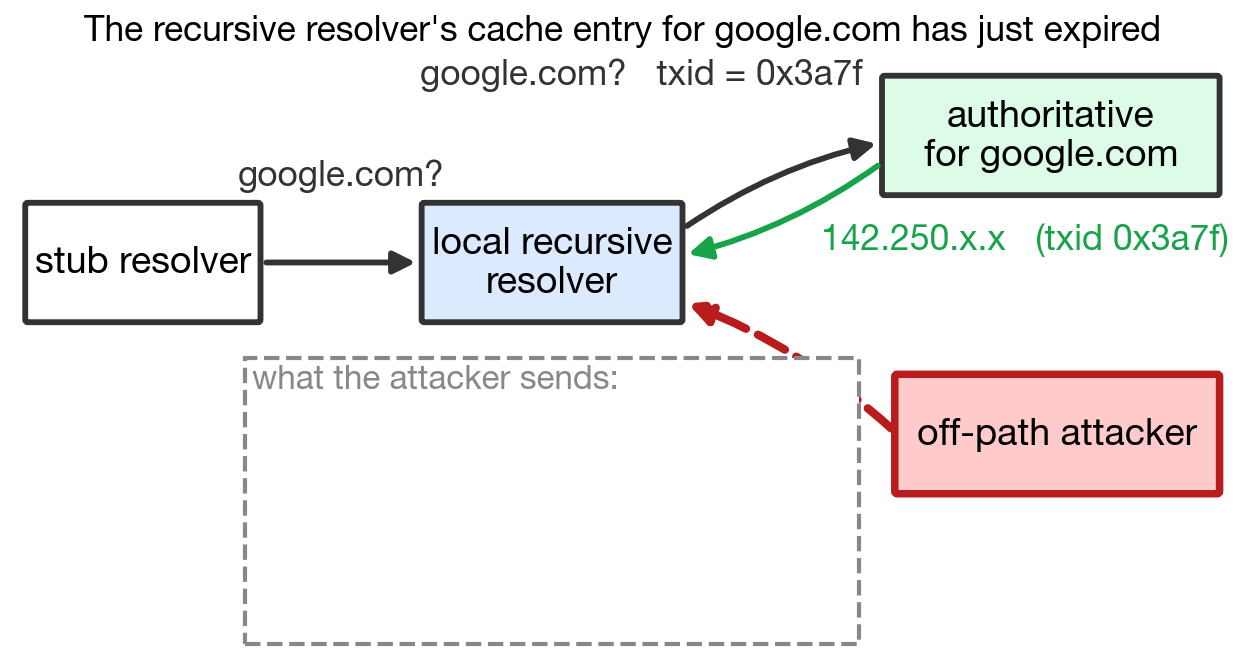
\includegraphics[width=\linewidth]{kaminsky.png}%
}
\end{minipage}
\eprob
\end{minipage}\par

\vspace*{-0.1in}
\section*{Course Feedback}
\vspace*{-0.25in}
\par\noindent\begin{minipage}{\linewidth}
\prob{1}
Interest (1=Boring!; 10=Amazing!): \gridbox{1.2cm}{0.8cm}{8}
Difficulty (1=Too easy; 10=Too hard): \gridbox{1.2cm}{0.8cm}{6}
\eprob
\end{minipage}\par
\par\noindent\begin{minipage}{\linewidth}
\prob{1}
(a) One thing you liked about the course so far. (b) One suggestion for
improvement:\\
\answerbox{1.6}{The debates. More time on the hands-on activities.}
\eprob
\end{minipage}\par
